\documentclass{article}
    \usepackage{amssymb}
    \usepackage{color}
    \usepackage{listings}
    \usepackage{graphicx}
    \usepackage{subcaption}
    \usepackage{geometry}
    \usepackage{float}
    \usepackage{caption}
    \usepackage{blindtext}
    \geometry{
    a4paper,
    total={170mm,257mm},
    left=20mm,
    top=20mm,
    }
    \DeclareCaptionFormat{citation}{%
    \ifx\captioncitation\relax\relax\else
      \captioncitation\par
    \fi
    #1#2#3\par}
 \newcommand*\setcaptioncitation[1]{\def\captioncitation{\textit{Source:}~#1}}
 \let\captioncitation\relax
 \captionsetup{format=citation,justification=centering}

    \setlength{\parindent}{0em}
    \setlength{\parskip}{1em} % length of the spacing
    
    \lstset{ % General setup for the package
        language=Python,
        basicstyle=\small\sffamily,
        numbers=left,
        numberstyle=\tiny,
        frame=tb,
        tabsize=4,
        columns=fixed,
        showstringspaces=false,
        showtabs=false,
        keepspaces,
        commentstyle=\color{red},
        keywordstyle=\color{blue},
        emphstyle=\ttb\color{deepred},    
        stringstyle=\color{deepgreen}
    }
    
    \begin{document}

    \begin{titlepage}
        \begin{center}
            \vspace*{1cm}
            \begin{figure}
                \centering
                
\includegraphics[width=0.5\linewidth]{./img/vub.png}
            \end{figure}
            \Huge
            \textbf{Distrinute Computing}
            
           
            
            \vspace{1.5cm}

            \textbf{Redona}
            \vspace{0.5cm}
            \textbf{Juan Jose Soriano Escobar}
            
            \vfill
            
            
            \Large
            Master in Applied Computer Science\\
            Vrije Universiteit Brussel\\
            Brussels Belgium\\
            January 15, 2017
            
        \end{center}
    \end{titlepage}

    \tableofcontents
    \newpage

    \begin{appendix}
        \listoffigures
      \end{appendix}
      \newpage


        \section{Introduction}
        \section{Implementation Architecture}
        As part of the implementation, we tried to go further with the implementation, combining concepts learn in previous courses of the master, such as Web technologies and Databases.  
        Our simulation pretends to simulate a "real case" environment, where several devices with different applications or back-end (e.g. mobile application in Python and web application in Nodejs)
        are used to collect an specific information and saved it in a pre-defined database.

        In the Figure \ref{} the global implementation is Illustrated. At the bottom level, it presents how two different application in Python and Nodejs uses the Twitter API to recollect and save tweets
        in an MongoDB database. The idea behind this implementation is to illustrate how information could be retrieve from different sources and be processed as one data source.
        Consequently, the information is save in a MongoDB database in an Amazon Web Server that would be later connected with Hadoop distributed storage.

        At the same time, in Amazon Web server are three EC2 instances running with Hadoop with one Name Node as a master, assigning work to two slave nodes working as Data nodes to process the MapReduce task in
        parallel. Finally to create the MapReduce job, PIG framework (cite??) was implemented and installed in the name node as high-level platform which allows to use MapReduce tasks in a simple way, implementing
        a familiar SQL syntax.

        Finally the results are stored in the namenode server and displayed in short HTML file.

        
        \section{Application layer}

        The application layer is the logic write in Python and in JavaScript to use the the Twitter API and save the data in the database. In order to avoid the same implementation in two different programming languages,
        we decided to implement the solutions in two different scenarios. One implementing JavaScript without data processing and a second solution with Python to with the respective data cleaning and preprocessing, to
        visualize how the results of the top ten words and hashtags may change with a "clean" and "noisy" data.

        The code implemented for the Python implementation can be find in the github repository: % add description?

        The code implemented for the Nodejs implementation can be find in the github repository: % add description?

        \subsection{Data Pre-processing}

        The data preprocessing is made by a function that receives the the streamed tweet from the tweetwe API and in a first place in tokenize the tweet in words, to later remove the stop words, special characters, links
        re-tweets and user tags, in order to extract the main words that potentially represent the meaning or topic of the tweet. Aditionally, Lemmatization is applied in the line \textit{13} to convert every word to the root 
        form, with the goal of grouping all the words that could semantically mean the same.
        \begin{lstlisting}[language=Python, caption= Tweet cleaning function, label={lst:dataCleaning}]
            def cleanTweet(tweet):    
                wordnet_lemmatizer = WordNetLemmatizer()
                stop = set(stopwords.words('english'))
                framents = tknz.tokenize(tweet)
                clean_fragments = []
                for f in framents:
                    if f not in stop: # not included in the stop words
                        f = f.lower() # lowercase word
                        f = re.sub(r'[.,"!~_:|?]+', '', f,flags=re.MULTILINE)
                        f = re.sub(url_expression, '', f,flags=re.MULTILINE) 
                        f = re.sub(r'@[a-z,A-Z,0-9 ]*', '', f, flags=re.MULTILINE) 
                        f = re.sub(r'RT @[a-z,A-Z]*: ', '', f, flags=re.MULTILINE) 
                        f = wordnet_lemmatizer.lemmatize(f)
                        if f:
                            clean_fragments.append(f)
                return(" ".join(clean_fragments))
        \end{lstlisting}

        \subsection{Twitter API Implementation}

        Implementation in Python....

        Implementation in Nodejs.....
        \section{Server Configuration}

        As  explained in section "look up" and presented in the Figure \ref{}, the server consist of one name node and two data nodes running in different Linux instances in Amazon Web Services.

        Besides the security rules and after the Hadoop and Java installation, it is important to configure five files:
            \begin{itemize}
                \item \textbf{hadoop-env.sh:} This file contains some environment variable settings used by Hadoop. Frequenly use these to modify some aspects of Hadoop daemon behavior, such as where 
                log files are stored, the maximum amount of heap used etc.                
                \item \textbf{core-site.xml:} contains the configuration of the name node and the temporal folder where the data is stored during the MapReduce process.
                \item \textbf{hdfs-site.xml:} contains the configuration for HDFS daemons, the NameNode, SecondaryNameNode  and data nodes.
                \item \textbf{mapred-site.xml:} contains the configuration settings for MapReduce daemons; it only need to specify in Hadoop that the yarn framework will be use for the map‐reduce jobs.
                \item \textbf{yarn-site.xml:} the properties in this file specify where the ResourceManager is running so that other processes can connect to it.
            \end{itemize}
        All the configuration files could be find in the github repository .....
        \begin{figure}[H]
            \centering 
            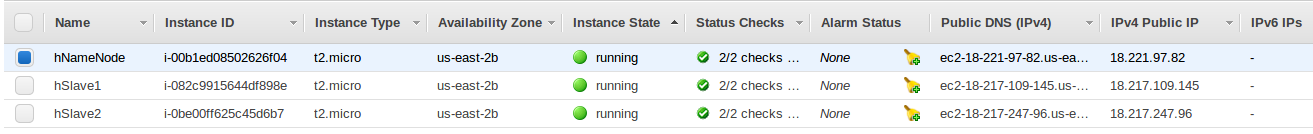
\includegraphics[width=1\linewidth]{./img/instances.png}
            \setcaptioncitation{Screenshot idk.}
            \caption{AWS instances.}
            \label{fig:instances}
        \end{figure}
        \section{MapReduce Job}

        To build the MapReduce Job, Apache Pig was used to take advantage of it easy SQL oriented approach to program, increasing the productivity and friendly for programmers that have not use Java before.
        Ten line of code in Pig Latin are equivalent almost to 200 lines of code in Java. (http://blog.cloudera.com/wp-content/uploads/2010/01/IntroToPig.pdf)

        Apache Pig is then installed in the name node and connected to YARN to manage the job request. 
        
        In the listing \ref{} is provided the job use to calculate the top ten used words and the top ten hashtags. From a global overview, the COUNT in Apache Pig is equivalent to a reduce and the Filter is translated to a map.
        Additionally the tokenize also represent a  map function that split a string of words into a bag of words.

        \begin{lstlisting}[caption= Tweet cleaning function, label={lst:dataCleaning}]
            REGISTER /home/ubuntu/hadoop/share/hadoop/common/lib/mongo-java-driver-3.6.0.jar;
            REGISTER /home/ubuntu/hadoop/share/hadoop/common/lib/mongo-hadoop-pig-2.0.2.jar;
            REGISTER /home/ubuntu/hadoop/share/hadoop/common/lib/mongo-hadoop-core-2.0.2.jar;
            
            data = LOAD '/home/ubuntu/distributedComputing/tweets.bson'
                USING
                com.mongodb.hadoop.pig.BSONLoader('fullResponse','text') AS (text:chararray);
            
            words = FOREACH data  GENERATE FLATTEN(TOKENIZE(text)) as word;
            grouped = GROUP words BY word;
            wordcount = FOREACH grouped GENERATE group, COUNT(words);
            
            ordered = ORDER wordcount by $1 DESC;
            top_words = LIMIT ordered 10;
            hash_filter = FILTER ordered BY $0 MATCHES '.*\\#\\p{Alpha}.*?';
            
            top_hash = LIMIT hash_filter 10;

            STORE top_hash INTO '/home/ubuntu/pig/scripts/top_10_hash';
            STORE top_words INTO '/home/ubuntu/pig/scripts/top_10_words'

        \end{lstlisting}

        The first three register statements in the Pig Script is implementing the Java, MongoDB and Hadoop conetors to work across the the architecture defined for the 3 instances. Then
        the BSON file from the database is loaded and the tweet is saved as "text". In the following lines, the tokenize divides the tweets into words (map) to consequently group them.
        From that point it is needed to count the amount of times that a word is present in the all the tweets, using COUNT (filter).
        
        With the pair word and number of repetitions of the word, is just matter of order them in descended order to identify the top ten words and filter (reduce) all the words that start by the character "#" to 
        extract also the top ten hashtags.

        Finally with the STORE command, the results are locally saved in the server.

        ** Apache Pig is a platform for analyzing large data sets that consists of a high-level language for expressing data analysis programs, coupled with infrastructure for evaluating these programs. 
        The salient property of Pig programs is that their structure is amenable to substantial parallelization, which in turns enables them to handle very large data sets. 
        (https://pig.apache.org/)

        ** YARN is the architectural center of Hadoop that allows multiple data processing engines such as interactive SQL, real-time streaming, data science and batch processing to handle data stored 
        in a single platform, unlocking an entirely new approach to analytics.
        https://hortonworks.com/apache/yarn/
        \section{Job Results}
        \section{Conclusion}

        \bibliography{report}
        \bibliographystyle{ieeetr}
        \nocite{*}

    \end{document}